\documentclass{beamer}
\usepackage{listings}
\lstset{
%language=C,
frame=single, 
breaklines=true,
columns=fullflexible
}
\usepackage{subcaption}
\usepackage{url}
\usepackage{amsmath}

\usepackage{amsthm}

\usepackage{tikz}
\usepackage{graphicx}
\usepackage{tkz-euclide} % loads  TikZ and tkz-base
%\usetkzobj{all}
\usetikzlibrary{calc,math}
\usepackage{float}

\newcommand\norm[1]{\left\lVert#1\right\rVert}
\renewcommand{\vec}[1]{\mathbf{#1}}
\newcommand{\R}{\mathbb{R}}
\newcommand{\C}{\mathbb{C}}
\providecommand{\brak}[1]{\ensuremath{\left(#1\right)}}
\providecommand{\abs}[1]{\vert#1\vert}
\providecommand{\fourier}{\overset{\mathcal{F}}{ \rightleftharpoons}}
\newcommand{\myvec}[1]{\ensuremath{\begin{pmatrix}#1\end{pmatrix}}}
\providecommand{\mean}[1]{E[ #1 ]}
\providecommand{\sbrak}[1]{\ensuremath{{}\left[#1\right]}}
\providecommand{\cbrak}[1]{\ensuremath{\left\{#1\right\}}}

\newcounter{saveenumi}
\newcommand{\seti}{\setcounter{saveenumi}{\value{enumi}}}
\newcommand{\conti}{\setcounter{enumi}{\value{saveenumi}}}

\usepackage[export]{adjustbox}
\usepackage[utf8]{inputenc}
\usepackage{amsmath}
\usetheme{Boadilla}
\title{Detection for Hybrid Beamforming Millimeter Wave Massive MIMO Systems}
\author{Raghav Juyal}
\date{EP20BTECH11018}
\begin{document}

\begin{frame}
\titlepage
\end{frame}
\begin{frame}{Aim}
    The aim of this paper is to improve the error performance
    of hybrid beamforming millimeter wave (mmWave) massive
    multi-input multi-output (MIMO) systems by designing detectors
    for such systems. 
\end{frame}

\begin{frame}{Abstract}
\begin{enumerate}
    \item Discuss the effect of the mmWave
channel parameters and hybrid beamforming settings on the
equivalent channel, which consists of the precoder, mmWave
channel, and combiner.
    \item Propose a low-complexity near-optimal signal detection scheme for the equivalent channel.
    \item Using computer simulations, it is shown that the error performance can be significantly improved and computational complexity reduced compared to other MIMO detection schemes.
\end{enumerate}

\end{frame}

\begin{frame}{Introduction}
\begin{enumerate}
    \item The majority of hybrid beamforming designs are based on the approach of approximating the optimal fully digital beamformer.
    
    \item The closeness of the hybrid beamformers to the optimal fully digital one is measured by the Euclidean distance.
    
    \item The effectiveness of the Euclidean distance for approximating the optimal beamformer in terms of spectral efficiency does not directly imply its efficacy in terms of more-practical metrics. 
    \item One reason is that the spectral efficiency performance theoretically depends on the largest eigenvalues of the channel, whereas the error performance is practically dictated by the stream with the lowest signal-to-noise ratio (SNR). Therefore, the approximation error can aggravate the error performance.
\end{enumerate}
\end{frame}

\begin{frame}{System Model}
    \begin{figure}[htp]
    \centering
    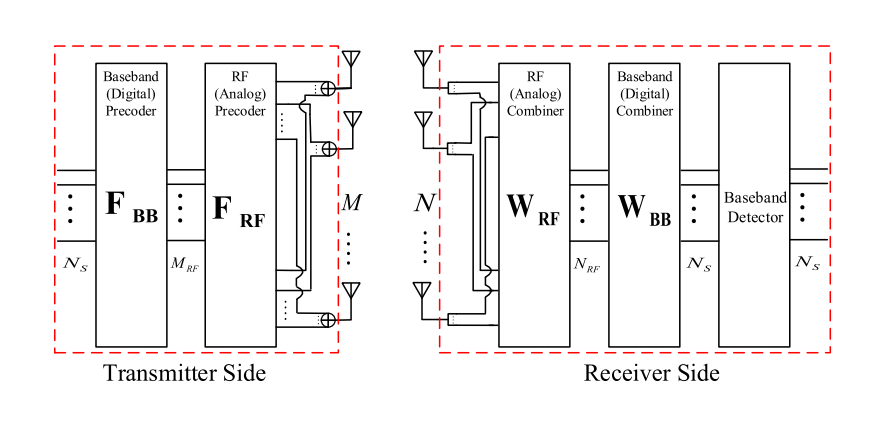
\includegraphics[width=10cm]{Fig_1.png}
    \caption{Fig. 1. System model of hybrid beamforming and detection for mmWave
massive MIMO systems}
    \label{Fig. 1.}
\end{figure}
\end{frame}

\begin{frame}{System Model Contd.} 
The entries of the data vector \textbf{s}, which is of size $N_S \times 1$, are chosen from a given constellation $\chi$, where 
\begin{align}
    \mathbb{E} [\boldsymbol{ss}^H] = \frac{1}{N_S} \boldsymbol{I}_{N_S}
\end{align}
The data vector is processed by a digital (baseband) precoder $\boldsymbol{F}_{BB}$ of size $M_{RF} \times N_S$ followed by an analog (RF) precoder $\boldsymbol{F}_{RF}$ of size $M \times M_{RF}$. Therefore, the vector \textbf{x}= $\boldsymbol{F}_{RF} \boldsymbol{F}_{BB} \boldsymbol{s}$ is sent over the channel.
The received vector of size $N\times 1$ is given by
\begin{align}
    \boldsymbol{y} = \sqrt{\rho}\boldsymbol{HF}_{RF}\boldsymbol{F}_{BB}\boldsymbol{s}+\boldsymbol{n}
\end{align}
where $\rho$ is the average received power and \textbf{n} is the white Gaussian noise vector with $\mathcal{CN}\brak{0,N_0}$ i.i.d. entries.
\end{frame}

\begin{frame}{System Model Contd.}
 \textbf{H} is
the fading channel matrix, which is modeled by the clustered model
\begin{align}
    \boldsymbol{H} = \sqrt{\frac{M\,N}{N_{cl}\,N_{ray}}} \sum_{i=1}^{N_{cl}} {\sum_{j=1}^{N_{ray}} {\alpha_{il} \boldsymbol{a}_r\brak{\phi_{il}^r,\theta_{il}^r} \boldsymbol{a}_t\brak{\phi_{il}^r,\theta_{il}^r}^H}}
\end{align}
where $N_{cl}$ is the number of clusters, and $N_{ray}$ is the number of contributing rays in each cluster. Hence, the total number
of paths is $L = N_{cl}N_{ray} $. Moreover, $\alpha_{il}$ is the complex gain of the \textit{j}-th ray in the \textit{i}-th cluster, and $\boldsymbol{a}_t\brak{\phi_{il}^r,\theta_{il}^r}$ is the transmit antenna array response vector of length $M$ for given azimuth and elevation angles of departure, respectively, denoted by
$\phi_{il}^t$ and $\theta_{il}^t$.
\end{frame}


\begin{frame}{System Model Contd.}
Similarly, $\boldsymbol{a}_r\brak{\phi_{il}^r,\theta_{il}^r}$ is the receive antenna array response vector of length $N$ for given azimuth and elevation angles of arrival. We  assume that the received signal is processed by $\boldsymbol{W}_{RF}$, i.e., the analog combiner, then by $\boldsymbol{W}_{BB}$, the digital combiner, and thereby the output of combiners is
\begin{align}
    \Tilde{\boldsymbol{y}} = \sqrt{\rho}\boldsymbol{W}_{BB}^H\boldsymbol{W}_{RF}^H\boldsymbol{HF}_{RF}\boldsymbol{F}_{BB}\boldsymbol{s}+\boldsymbol{W}_{BB}^H\boldsymbol{W}_{RF}^H\boldsymbol{n}
\end{align}
After that, the signal combining stage is followed by a
detection stage that estimates the transmitted data vector.
\end{frame}
 
\begin{frame}{}
\begin{center}
    PROPOSED SIGNAL DETECTION ALGORITHM
\end{center}
\end{frame}

\begin{frame}{Equivalent Channel Matrix}
  We consider the equivalent channel consisting of the precoder, mmWave channel, and combiner, i.e.,
  \begin{align}
      \boldsymbol{H}_{eq} = \boldsymbol{W}^H\boldsymbol{HF} \label{eq1}
  \end{align}
  for the detection process. Hence, we have
  \begin{align}
      \Tilde{y} = \sqrt{\rho}\boldsymbol{H}_{eq}\boldsymbol{s}+\boldsymbol{n'}
  \end{align}
  where $ \boldsymbol{n'} = \boldsymbol{W}^H\boldsymbol{n}$.\\ In practical mmWave massive MIMO systems, the number of data streams, i.e., $N_S$ is as high as 8. Because of
the near-diagonal structure of the equivalent channel in \eqref{eq1}, it is expected that MIMO detection techniques such as the fixed-complexity sphere decoder (FSD) and the subspace
detection scheme in can be extensively simplified by exploiting the structure.
\end{frame}

\begin{frame}{Proposed Low-Complexity Near-Optimal Detector}
\begin{figure}[htp]
    \centering
    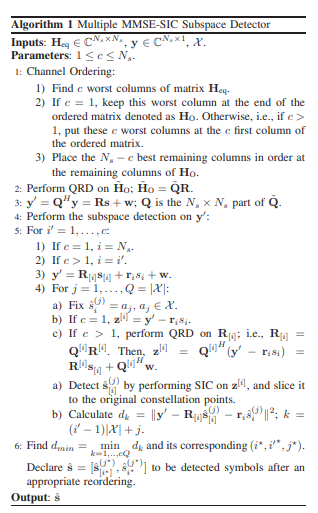
\includegraphics[width=4.75cm]{Fig_2.png}
\end{figure}
\end{frame}

\begin{frame}{}
  The proposed detector consists of the following steps:
  \begin{enumerate}
      \item Channel Ordering:  We consider the regularized
    (or augmented) channel matrix, i.e.,
    \begin{align}
        \Tilde{\boldsymbol{H}}_{eq} = \left[ \frac{\boldsymbol{H}_{eq}}{\sqrt{\alpha}\boldsymbol{I}_{N_S}} \right]
    \end{align}
    where $\alpha = \frac{N_o}{\rho}$. Depending on the value of $c$, which is the number of columns that are considered for subspace detection step, an appropriate channel ordering is performed, and the ordered matrix is denoted as $\boldsymbol{H}_O$.
    \seti
  \end{enumerate}
\end{frame}

\begin{frame}{}
    \begin{enumerate}
    \conti
    \item MMSE(minimum mean square error) Filtering: We perform the QR decomposition (QRD)
    on $\boldsymbol{H}_O$, i.e.,
    \begin{align}
         \Tilde{\boldsymbol{H}}_{O} = \Tilde{\boldsymbol{Q}}\boldsymbol{R}
    \end{align}
    where $\Tilde{\boldsymbol{Q}}$ is an $2N_S \times N_S$ matrix with orthonormal columns, and $\boldsymbol{R}$ is an $N_S \times N_S$ upper-triangular matrix with positive diagonal entries.
        By considering $\boldsymbol{Q}$ as the first $N_S$ rows of $\Tilde{\boldsymbol{Q}}$ one writes
        \begin{align}
            \boldsymbol{y'} = \boldsymbol{Q}^H\boldsymbol{y} = \boldsymbol{Rs}+\boldsymbol{w}
        \end{align}
        where $\boldsymbol{w} = \boldsymbol{Q}^H\boldsymbol{n'} - \left[ \boldsymbol{R} - \boldsymbol{Q}^H\boldsymbol{H}_{eq} \right]\boldsymbol{s}$ 
        \seti
    \end{enumerate}
\end{frame}

\begin{frame}{}
    \begin{enumerate}
        \conti
        \item Subspace Detection: The idea of subspace detection is to divide the symbol vector into two subvectors. Here, we consider a subvector of size one for the detection of one symbol corresponding to one column. Hence, we have
        \begin{align}
            \boldsymbol{y'} = \boldsymbol{R}_{[i]}\boldsymbol{s}_{[i]}+\boldsymbol{r}_is_i+\boldsymbol{w}
        \end{align}
        where $\boldsymbol{R}_{[i]}$ is the submatrix of $\boldsymbol{R}$ obtained by removing the \textit{i}-th column. The constellation points are searched to find $s_i$. When $c>1$, we examine $c$ worst columns in a round-robin fashion for subspace detection.
        \seti
    \end{enumerate}
\end{frame}

\begin{frame}{}
    \begin{enumerate}
        \conti
        \item Successive Interference Cancellation (SIC): After removing the affect of each considered constellation point, SIC is performed to detect the remaining symbols. If $c=1$, $\boldsymbol{r}_{N_S}$ is used for subspace detection. Hence, SIC is performed using the upper-triangular structure of $\boldsymbol{R}_{[N_S]}$. However, when $c>1$, a second QRD is required in order for $\boldsymbol{R}_{[i]}$ to have an upper-triangular form for SIC. 
    \end{enumerate}
\end{frame}

\begin{frame}{Computational Complexity}
In Algorithm 1, QRD and the channel ordering both require $\mathcal{O}(N_S^3)$ operations. For multiple subspace detection, additional $\mathcal{O}(cN_S^2)$ operations are required for all second QRDs. Table I shows the detailed complexity of the proposed algorithm in terms of number of floating-point operations (FLOPs) assuming six and two FLOPs per complex multiplication and addition, respectively. The complexity of the proposed algorithm is $\mathcal{O}(N_S^3|\chi|)$.
\begin{figure}[htp]
    \centering
    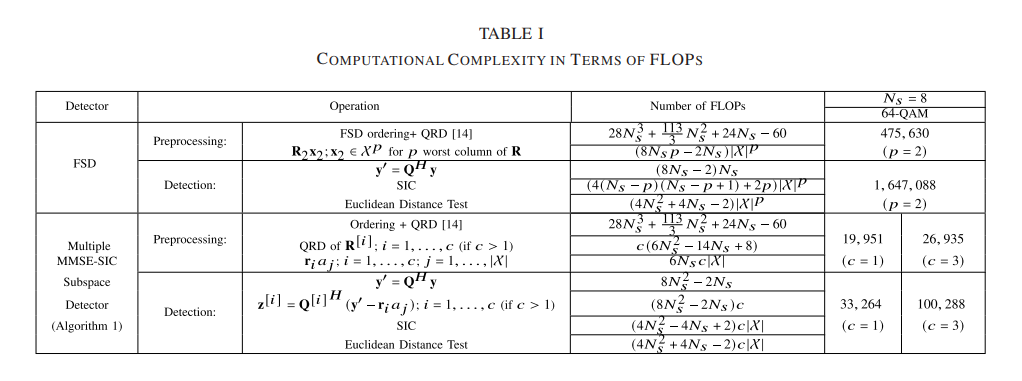
\includegraphics[width=12cm]{Fig_3.png}
\end{figure}
\end{frame}

\begin{frame}{Simulation Results}
    \begin{figure}[htp]
    \centering
    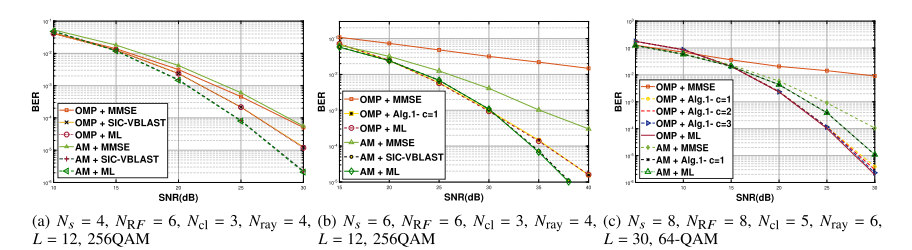
\includegraphics[width=12cm]{Fig_4.png}
    \caption{Fig. 2. BER of hybrid beamforming with detection for a 64 × 16 UPA mmWave massive MIMO System}
    \label{Fig. 2.}
\end{figure}
\end{frame}

\begin{frame}{Conclusion}
\begin{enumerate}
    \item The approximation error introduced to mmWave massive
    MIMO systems due to hybrid beamforming techniques can
    significantly degrade the error performance of these systems.
    \item The proposed  signal detection algorithm  can improve the error performance of such systems.
    \item The proposed algorithm approaches the error performance of
    the optimal ML detector, while also reducing the computational complexity compared to the ML or other conventional detectors.
\end{enumerate}
\end{frame}

\end{document}